%% abtex2-modelo-trabalho-academico.tex, v-1.7.1 laurocesar
%% Copyright 2012-2013 by abnTeX2 group at http://abntex2.googlecode.com/ 
%%
%% This work may be distributed and/or modified under the
%% conditions of the LaTeX Project Public License, either version 1.3
%% of this license or (at your option) any later version.
%% The latest version of this license is in
%%   http://www.latex-project.org/lppl.txt
%% and version 1.3 or later is part of all distributions of LaTeX
%% version 2005/12/01 or later.
%%
%% This work has the LPPL maintenance status `maintained'.
%% 
%% The Current Maintainer of this work is the abnTeX2 team, led
%% by Lauro César Araujo. Further information are available on 
%% http://abntex2.googlecode.com/
%%
%% This work consists of the files abntex2-modelo-trabalho-academico.tex,
%% abntex2-modelo-include-comandos and abntex2-modelo-references.bib
%%

% ------------------------------------------------------------------------
% ------------------------------------------------------------------------
% abnTeX2: Modelo de Trabalho Academico (tese de doutorado, dissertacao de
% mestrado e trabalhos monograficos em geral) em conformidade com 
% ABNT NBR 14724:2011: Informacao e documentacao - Trabalhos academicos -
% Apresentacao
% ------------------------------------------------------------------------
% ------------------------------------------------------------------------


%%%%%%%%%%%%%%%%%%
%
% As alterações realizadas no leiaute original do abntex2 disponibilizado 
% no sharelatex adaptaram o leiaute do abntex2 aos requisitos mínimos
% para escrita de dissertações e teses customizadas para o 
% centro de informática da ufpe.
%
% Bruno Maciel <bifm@cin.ufpe.com> 20/10/2016
% Daniel Severo Estrázulas <dse@cin.ufpe.br> 19/10/2020
% Alterações realizadas para o template da biblioteca atualizado disponibilizado no site Versão 07.10.2020 (1.3) revisado pelas bibliotecárias do setor bibccen.pt@ufpe.br
%%%%%%%%%%%%%%%%%%%%%%%%%%%%%%%%%%%%%%%%%%%%%%%%%%%%%%%%%%%%%%%

\documentclass[
	% -- opções da classe memoir --
	12pt,				% tamanho da fonte
	openright,			% capítulos começam em pág ímpar (insere página vazia caso preciso)
	oneside,			% para impressão em verso e anverso. Oposto a oneside
	a4paper,			% tamanho do papel. 
	% -- opções da classe abntex2 --
	chapter=TITLE,		% títulos de capítulos convertidos em letras maiúsculas
	section=TITLE,		% títulos de seções convertidos em letras maiúsculas
	%subsection=TITLE,	% títulos de subseções convertidos em letras maiúsculas
	%subsubsection=TITLE,% títulos de subsubseções convertidos em letras maiúsculas
	% -- opções do pacote babel --
	%english,			% idioma adicional para hifenização
	french,				% idioma adicional para hifenização
	spanish,			% idioma adicional para hifenização
%	brazil,				% o último idioma é o principal do documento
	english,
	brazil,
	]{abntex2/abntex2}
	\renewcommand{\baselinestretch}{1.5} %para customizar o espaço entre as linhas do texto
% --
% SETTINGS

\usepackage{abntex2/abntex2-cin-ufpe}

% \usepackage[noframe]{showframe}
% \usepackage{showframe}

%\overfullrule=4mm %para identificar onde existem os alertas de linhas grandes mal formatada pelo LaTex, basta comentar para não aparecer a barra lateral preta na linha em questão.

\renewcommand*\arraystretch{1.2} %para customizar o espaço entre as linhas das tabelas


\usepackage{pdfpages} %para incluir pdf como páginas


% ---
% PACOTES
% ---
\usepackage{float}
\usepackage{cmap}				% Mapear caracteres especiais no PDF
\usepackage{lmodern}			% Usa a fonte Latin Modern			
\usepackage[T1]{fontenc}		% Selecao de codigos de fonte.
\usepackage[utf8]{inputenc}		% Codificacao do documento (conversão automática dos acentos)
\usepackage{lastpage}			% Usado pela Ficha catalográfica
\usepackage{indentfirst}		% Indenta o primeiro parágrafo de cada seção.
%\usepackage{color}				% Controle das cores
\usepackage{graphicx}			% Inclusão de gráficos
\usepackage{lipsum}				% para geração de dummy text
\usepackage[versalete,alf,abnt-and-type=e,abnt-etal-list=0,abnt-etal-cite=3]{abntex2/abntex2cite} 
\usepackage{multirow}
\usepackage[section]{placeins}



% -----------------------------------------------------------
% lista de abreviaturas e siglas
% início
% -----------------------------------------------------------
% \usepackage[noredefwarn,acronym]{glossaries} %GLOSSÁRIO
\usepackage[acronym,nonumberlist,nogroupskip,noredefwarn]{glossaries}
% \usepackage{glossary-superragged}

\newcolumntype{L}[1]{>{\raggedright\let\newline\\\arraybackslash\hspace{0pt}}m{#1}}
\newcolumntype{C}[1]{>{\centering\let\newline\\\arraybackslash\hspace{0pt}}m{#1}}
\newcolumntype{R}[1]{>{\raggedleft\let\newline\\\arraybackslash\hspace{0pt}}m{#1}}

\newglossarystyle{modsuper}{%
  \glossarystyle{super}%
  \renewcommand{\glsgroupskip}{}
  
  % put the glossary in a longtable environment:
 \renewenvironment{theglossary}%
  {
    \begin{longtable}
        {L{0.2\textwidth}L{0.8\textwidth}}}%
    {\end{longtable}
  }%
}

% -----------------------------------------------------------
% lista de abreviaturas e siglas
% fim
% -----------------------------------------------------------


\usepackage{lscape} 
\usepackage{rotating} %rotates the figures, page
\usepackage{tikz}
\usepackage[section]{placeins}
\usepackage{setspace} 



% ----------------------------------------------------------
% PERSONALIZAÇÃO DE CORES
% ----------------------------------------------------------
\definecolor{blue}{RGB}{41,5,195}
\definecolor{gray}{rgb}{.4,.4,.4}
\definecolor{gray}{rgb}{.4,.4,.4}
\definecolor{pblue}{rgb}{0.13,0.13,1}
\definecolor{pgreen}{rgb}{0,0.5,0}
\definecolor{pred}{rgb}{0.9,0,0}
\definecolor{pgrey}{rgb}{0.46,0.45,0.48}
\definecolor{lightgray}{rgb}{0.95, 0.95, 0.96}
\definecolor{whitesmoke}{rgb}{0.96, 0.96, 0.96}
\definecolor{javared}{rgb}{0.6,0,0} % for strings
\definecolor{javagreen}{rgb}{0.25,0.5,0.35} % comments
\definecolor{javapurple}{rgb}{0.5,0,0.35} % keywords
\definecolor{javadocblue}{rgb}{0.25,0.35,0.75} % javadoc
\definecolor{meucinza}{rgb}{0.5, 0.5, 0.5}
%\definecolor{lightgray}{gray}{0.9}


% ----------------------------------------------------------
% PERSONALIZAÇÃO DO USUÁRIO
% ----------------------------------------------------------
\input{custom}


% ----------------------------------------------------------
% COMPILA O ÍNDICE
% ----------------------------------------------------------
\makeindex
% ---


% ----------------------------------------------------------
% LISTA E ABREVIATURAS E SIGLAS
% ----------------------------------------------------------
% Lista de acrônimos:
\newacronym{oms}{OMS}{Organização Mundial da Saúde}
\newacronym{cfm}{CFM}{Conselho Federal de Medicina}
\newacronym{ibge}{IBGE}{Instituto Brasileiro de Geografia e Estatística}
\newacronym{ines}{INES}{Instituto Nacional de Educação de Surdos}
\newacronym{slr}{RLS}{Reconhecimento de Língua de Sinais}
\newacronym{ia}{IA}{Inteligência Artificial}
\newacronym{nlp}{PLN}{Processamento de Linguagem Natural}
\newacronym{mt}{TA}{Tradução Automática}
\newacronym{mhi}{MHI}{\textit{Motion History Image} (Imagem do Histórico de Movimento)}
\newacronym{mei}{MEI}{\textit{Motion Energy Image} (Imagem de Energia de Movimento)}
\newacronym{asllvd}{ASLLVD}{\textit{American Sign Language Lexicon Video Dataset}}
\newacronym{asllrp}{ASLLRP}{\textit{American Sign Language Linguistic Research Project}}
\newacronym{lstm}{LSTM}{\textit{Long Short-Term Memory}}
\newacronym{gru}{GRU}{\textit{Gated Recurrent Unit}}
\newacronym{rnn}{RNN}{\textit{Recurrent Neural Network} (Rede Neural Recorrente)}
\newacronym{cnn}{CNN}{\textit{Convolutional Neural Network} (Rede Neural Convolucional)}
\newacronym{ipa}{IPA}{\textit{International Phonetic Alphabet} (Alfabeto Fonético Internacional)}
\newacronym{sgd}{SGD}{\textit{Stochastic Gradient Descent
} (Gradiente Estocástico Descendente)}
\newacronym{pca}{PCA}{\textit{Principal Component Analysis
} (Análise de Componente Principal)}
\newacronym{hof}{HOF}{\textit{Histogram of Optical Flow
} (Histograma de Fluxo Óptico)}
\newacronym{hmm}{HMM}{\textit{Hidden Markov Model} (Modelos Ocultos de Markov)}
\newacronym{crf}{CRF}{\textit{Conditional Random Fields} 
(Campos Aleatórios Condicionais)}
\newacronym{cv}{VC}{Visão Computacional}
\newacronym{dl}{AP}{Aprendizagem Profunda}
\newacronym{ml}{AM}{Aprendizagem de Máquina}

% Línguas de sinais
\newacronym{asl}{ASL}{\textit{American Sign Language} (Língua de Sinais Americana)}
\newacronym{csl}{CSL}{\textit{Chinese Sign Language} (Língua de Sinais Chinesa)}
\newacronym{dgs}{DGS}{\textit{Deutsche Gebärdensprache} (Língua de Sinais Alemã)}
\newacronym{bsl}{BSL}{\textit{British Sign Language} (Língua de Sinais Britânica)}
\newacronym{arsl}{ArSL}{\textit{Arabic Sign Language} (Língua de Sinais Britânica)}
\newacronym{jsl}{JSL}{\textit{Japanese Sign Language} (Língua de Sinais Japonesa)}
\newacronym{isl}{ISL}{\textit{Indian Sign Language} (Língua de Sinais Indiana)}
\newacronym{gsl}{GSL}{\textit{Greek Sign Language} (Língua de Sinais Grega)}
\newacronym{tid}{TID}{\textit{Türk İşaret Dili} (Língua de Sinais Turca)}
\newacronym{ngt}{NGT}{\textit{Nederlandse Gebarentaal} (Língua de Sinais Holandesa)}
\newacronym{vgt}{VGT}{\textit{Vlaamse Gebarentaal} (Língua de Sinais Flamenga)}
\newacronym{lis}{LIS}{\textit{Lingua dei Segni Italiana} (Língua de Sinais Italiana)}
\newacronym{auslan}{AUSLAN}{\textit{Australian Sign Language} (Língua de Sinais Austrália)}
\newacronym{lsa}{LSA}{\textit{Lengua de Señas Argentina} (Língua de Sinais Argentina)}
\newacronym{tsl}{TSL}{\textit{Taiwan Sign Language} (Língua de Sinais de Taiwan)}
\newacronym{pjm}{PJM}{\textit{Polski Język Migowy} (Língua de Sinais Polonesa)}
\newacronym{libras}{Libras}{Língua Brasileira de Sinais}
\newacronym{tch}{TCH}{\textit{Teanga Chomharthaíochta na hÉireann} (Língua de Sinais Irlandesa)}
\newacronym{ksl}{KSL}{\textit{Korean Sign Language} (Língua de Sinais Coreana)}
\newacronym{bisindo}{BISINDO}{\textit{Bahasa Isyarat Indonesia} (Língua de Sinais Indonésia)}

\makenoidxglossaries
\renewcommand*{\glsseeformat}[3][\seename]{\textit{#1}  
\glsseelist{#2}}

\renewcommand*{\glspostdescription}{} % remove trailing dot
\renewcommand{\glsnamefont}[1]{\textbf{#1}}

\renewcommand{\familydefault}{\sfdefault}

% ----------------------------------------------------------
% GLOSSÁRIO
% ----------------------------------------------------------
\input{others/glossaries}


\usepackage{pdfpages}
\usepackage{inconsolata}
\usepackage{listings}

\definecolor{cinza}{HTML}{FCF8F8}

% define formato e estilo dos elementos do tipo Codigo Fonte
\lstset{language=PHP,
basicstyle=\ttfamily\scriptsize,
%basicstyle=\ttfamily,
keywordstyle=\color{javapurple}\bfseries,
stringstyle=\color{pblue},
commentstyle=\color{javagreen},
morecomment=[s][\color{javadocblue}]{/**}{*/},
morecomment=[s][\color{gray}]{@}{\ },
numbers=left,
numberstyle=\tiny\color{black},
backgroundcolor=\color{cinza},
stepnumber=2,
numbersep=8pt,
xleftmargin=14pt,
tabsize=4,
showspaces=false,
showstringspaces=false,
breaklines=true,}

%%%%%%%%%%%%%%%%%%%%%%%%%%%%%%%%%%



\usepackage{adjustbox} % ajustar tabela ao tamanho da pagina


% ----------------------------------------------------------
% INÍCIO DO DOCUMENTO
% ----------------------------------------------------------
\begin{document}

\frenchspacing % Retira espaço extra obsoleto entre as frases.

\imprimircapa
\imprimirfolhaderosto*~
%a ficha deve ser passada pelo setor da biblioteca e sobrescrito no formato pdf

\includepdf[pages=-]{others/ficha.pdf}

%\newpage
%% Ata de defesa

\includepdf[pages=-]{outros/biblioteca/ata_defesa.pdf}

%a folha de aprovação deve ser um pdf que a secretaria encaminha sem assinaturas
%basta fazer upload na basta others e sobrescrever

\includepdf[pages=-]{others/folha_aprovacao_original}

% ----------------------------------------------------------
% DEDICATÓRIA
% ----------------------------------------------------------
\begin{dedicatoria}
   \vspace*{\fill}
   % \centering
   % \noindent
   \textit{
      Dedico este trabalho ao meu pai, que partiu ao longo da jornada deste mestrado, mas que deixou um grande exemplo de integridade e simplicidade pelo qual me espelharei em minha caminhada.
   }
\end{dedicatoria}
% ---

% ----------------------------------------------------------
% AGRADECIMENTOS
% ----------------------------------------------------------
\begin{agradecimentos}
Texto texto texto texto texto texto texto texto texto texto texto texto texto texto texto texto texto texto texto texto texto texto texto texto texto texto texto texto texto texto texto texto texto texto texto texto texto texto texto texto texto texto.

Texto texto texto texto texto texto texto texto texto texto texto texto texto texto texto texto texto texto texto texto texto texto texto texto texto texto texto texto texto texto texto texto texto texto texto texto texto texto texto texto texto texto.

Texto texto texto texto texto texto texto texto texto texto texto texto texto texto texto texto texto texto texto texto texto texto texto texto texto texto texto texto texto texto texto texto texto texto texto texto texto texto texto texto texto texto.

Texto texto texto texto texto texto texto texto texto texto texto texto texto texto texto texto texto texto texto texto texto texto texto texto texto texto texto texto texto texto texto texto texto texto texto texto texto texto texto texto texto texto.



\end{agradecimentos}
% ----------------------------------------------------------
% EPÍGRAFE

%Epígrafe: Elemento opcional e sem título em que o (a) autor (a) apresenta uma citação relacionada ao assunto tratado no trabalho. Deve ser elaborada conforme a ABNT-NBR 10520 (Citações). As citações de até três linhas devem estar entre aspas duplas e as citações com mais de três linhas devem ser destacadas com recuo de 4 cm da margem esquerda, com letra menor que a do texto e sem as aspas. A fonte da citação deve aparecer na lista de referências.
% ---------------------------------------------------------
\vspace*{\fill}

\begin{citacao}
  ``Conheça todas as teorias, domine todas as técnicas, mas ao tocar uma alma humana seja apenas outra alma humana.''
  (Carl Gustav Jung)
\end{citacao}

\newpage
% -----------------------------------------------------------
% PORTUGUÊS
% -----------------------------------------------------------
\begin{resumo}[Resumo]
  \noindent
  A língua de sinais é uma ferramenta essencial na vida do Surdo, capaz de assegurar seu acesso à comunicação, educação e desenvolvimento cognitivo e socio-emocional.
  Na verdade, ela é a principal força que une essa comunidade e o símbolo de identificação entre seus membros.
  Contudo, atualmente o número de indivíduos ouvintes que conseguem se comunicar por meio dessa língua é pequeno e, na prática, isso impõe obstáculos ao cotidiano do Surdo.
  Tarefas simples como utilizar o transporte público, comprar roupas, ir ao cinema ou obter assistência médica acabam tornando-se um desafio por conta dessa limitação.
  O Reconhecimento de Língua de Sinais é uma das áreas de pesquisa que objetiva desenvolver tecnologias capazes de reduzir essas barreiras linguísticas e facilitar a comunicação entre ambos indivíduos.
  Apesar disso, ao analisar sua evolução ao longo das últimas décadas, percebe-se que seu progresso ainda não é suficiente para disponibilizar soluções efetivamente aplicáveis ao mundo real.
  Isso ocorre principalmente porque várias pesquisas na área acabam não apropriando-se ou abordando adequadamente as particularidades linguísticas das línguas de sinais, decorrentes de sua natureza visual.
  Tendo isso em vista, este trabalho apresenta uma abordagem que aplica modelos sequenciais de aprendizagem de máquina para realizar o reconhecimento computacional dos sinais através de seus atributos linguísticos. Além disso, são introduzidos dois novos \textit{datasets} para a língua de sinais, dentre os quais está um \textit{dataset} de atributos linguísticos computados a partir do ASLLVD.
  Com isso, objetiva-se estabelecer uma direção capaz de conduzir a avanços mais efetivos para essa área e, consequentemente, contribuir com a superação dos obstáculos hoje enfrentados pelo Surdo.

  \vspace{\onelineskip}

  \noindent
  \textbf{Palavras-chaves}: Língua de Sinais. Linguística. Processamento de Linguagem Natural.
\end{resumo}



% -----------------------------------------------------------
% INGLÊS
% -----------------------------------------------------------
\begin{resumo}[Abstract]
  \begin{otherlanguage*}{english}
    \noindent
    Sign language is an essential resource to ensure the Deaf to have access to communication, education, as well as to cognitive and socio-emotional development. In fact, it is the main force that unites such community and the key trait that identifies its members.
    On the other hand, the number of hearing individuals who are able to communicate through this language is currently small and, in practice, this imposes obstacles to the daily life of the Deaf.
    Simple tasks like using public transportation, shopping for clothes, going to the movies, or getting medical assistance end up becoming challenges due to such limitation.
    The Sign Language Recognition, in turn, is one of the research areas dedicated to developing technologies that aim to reduce such language barriers and facilitate the communication between these individuals.
    However, when analyzing its evolution over the last decades, we realize that it has not progressed enough to provide solutions effectively applicable to the real world.
    This is mainly because several researches in this field do not appropriate or address the linguistic particularities presented by the sign languages, which stem from their visual nature.
    Considering this problem, the present work introduces an approach that adopts sequential machine learning models to recognize signs through their linguistic attributes. In addition, we introduce two new sign language datasets, among which is a novel dataset of linguistic attributes computed from the ASLLVD.
    Thus, we aim to establish a direction that can lead to more effective advances in this research area and, consequently, contribute to overcoming the obstacles faced by the Deaf today.

    \vspace{\onelineskip}

    \noindent
    \textbf{Keywords}: Sign Language. Linguistics. Natural Language Processing.
  \end{otherlanguage*}
\end{resumo}



% ----------------------------------------------------------
% LISTA DE FIGURAS
% ----------------------------------------------------------
\pdfbookmark[0]{\listfigurename}{lof}
\listoffigures*
\cleardoublepage


% ---
% LISTA DE CÓDIGOS FONTES
% ---

\pdfbookmark[0]{\lstlistingname}{lol} % caso não tenha quadros, comente esta linha 
\counterwithout{lstlisting}{chapter}



% Altera o nome padrão do rótulo usado no comando \autoref{}
\renewcommand{\lstlistingname}{Código Fonte}

% Altera o rótulo a ser usando no elemento pré-textual "Lista de código"
\renewcommand{\lstlistlistingname}{Lista de códigos}

% Configura a ``Lista de Códigos'' conforme as regras da ABNT (para abnTeX2)
\begingroup\makeatletter
\let\newcounter\@gobble\let\setcounter\@gobbletwo
  \globaldefs\@ne \let\c@loldepth\@ne
  \newlistof{listings}{lol}{\lstlistlistingname}
  \newlistentry{lstlisting}{lol}{0}
\endgroup

\renewcommand{\cftlstlistingaftersnum}{\hfill--\hfil}

\let\oldlstlistoflistings\lstlistoflistings
{
\let\oldnumberline\numberline
\newcommand{\algnumberline}[1]{Código Fonte~#1~\enspace--~\enspace}
\renewcommand{\numberline}{\algnumberline}

\begin{KeepFromToc}
\lstlistoflistings
\end{KeepFromToc}
}
\cleardoublepage

% ---
% LISTA DE QUADROS
% ---
\pdfbookmark[0]{\listofquadrosname}{loq} % caso não tenha quadros, comente esta linha 
\listofquadros* % caso não tenha quadros, comente esta linha 
\cleardoublepage



% ----------------------------------------------------------
% LISTA DE TABELAS
% ----------------------------------------------------------

\pdfbookmark[0]{\listtablename}{lot}
\listoftables*
\cleardoublepage


        
  
% ----------------------------------------------------------
% LISTA E ABREVIATURAS E SIGLAS
% ----------------------------------------------------------
% \printglossary[type=\acronymtype,title={\listadesiglasname},nonumberlist]
% \printglossaries
% compile uma vez com o comando \printglossaries e depois compile novamente com o comando \printglossaries comentado para as páginas glossário e siglas serem ocultadas.

% ----------------------------------------------------------
% LISTA E ABREVIATURAS E SIGLAS
% ----------------------------------------------------------
% \setglossarystyle{modsuper}
\printnoidxglossary[style=modsuper,type=\acronymtype,title={\listadesiglasname},nonumberlist]
% \printglossary[style=super, type=\acronymtype]
\cleardoublepage



% ----------------------------------------------------------
% LISTA DE SIMBOLOS
% ----------------------------------------------------------



% ---

% ---
% inserir lista de símbolos
% ---
\begin{simbolos}
  \item[$ \gamma $] Letra grega Gama
  %\item[$ \Lambda $] Lambda
  %\item[$ \zeta $] Letra grega minúscula zeta
  \item[$ \in $] Pertence
%  \item[$ \infty$] Infinito
%  \item[$ \ge$] Maior ou Igual
  \item[$ \delta$] Delta
  \item[$ \theta$] Teta
  \item[$ \sigma$] Sigma
  \item[$ \mu$] Mi
  
\end{simbolos}
% ---




% ----------------------------------------------------------
%


% ---

% ---
% inserir lista de símbolos
% ---
\begin{simbolos}
  \item[$ \gamma $] Letra grega Gama
  %\item[$ \Lambda $] Lambda
  %\item[$ \zeta $] Letra grega minúscula zeta
  \item[$ \in $] Pertence
%  \item[$ \infty$] Infinito
%  \item[$ \ge$] Maior ou Igual
  \item[$ \delta$] Delta
  \item[$ \theta$] Teta
  \item[$ \sigma$] Sigma
  \item[$ \mu$] Mi
  
\end{simbolos}
% ---






% ----------------------------------------------------------
% SUMÁRIO
% ----------------------------------------------------------
\pdfbookmark[0]{\contentsname}{toc}
\tableofcontents*
% \begingroup\intoctrue
% \tableofcontents*
% \endgroup
\cleardoublepage

% \setcounter{page}{13}
\setcounter{tocdepth}{2}
\setcounter{table}{0}




% ----------------------------------------------------------
% ELEMENTOS TEXTUAIS
% ----------------------------------------------------------
\textual

\input{summary}

\bookmarksetup{startatroot}% 


% ----------------------------------------------------------
% ELEMENTOS PÓS-TEXTUAIS
% ----------------------------------------------------------
\postextual


% ----------------------------------------------------------
% Referências bibliográficas
% ----------------------------------------------------------
%\bibliographystyle{abntexalfenglish} %caso seja em inglês, retire o comentário desta linha

% \renewcommand{\bibname}{REFER\^ENCIAS}
%\renewcommand{\bibname}{Bibliography}
% \addbibresource{sample.bib}
\bibliography{references2}


% ----------------------------------------------------------
% Apêndices
% ----------------------------------------------------------


% ----------------------
% força para que não exiba subtítulos em apêndices no sumário
% -----------------------

\begin{apendicesenv}
\addtocontents{toc}{\protect\setcounter{tocdepth}{1}}
\makeatletter
\addtocontents{toc}{%
  \begingroup
  \let\protect\l@chapter\protect\l@section
  \let\protect\l@section\protect\l@subsection
}
\makeatother

% Imprime uma página indicando o início dos apêndices
% \partapendices

%coloca o identificador do anexo/apendice somente na primeira página
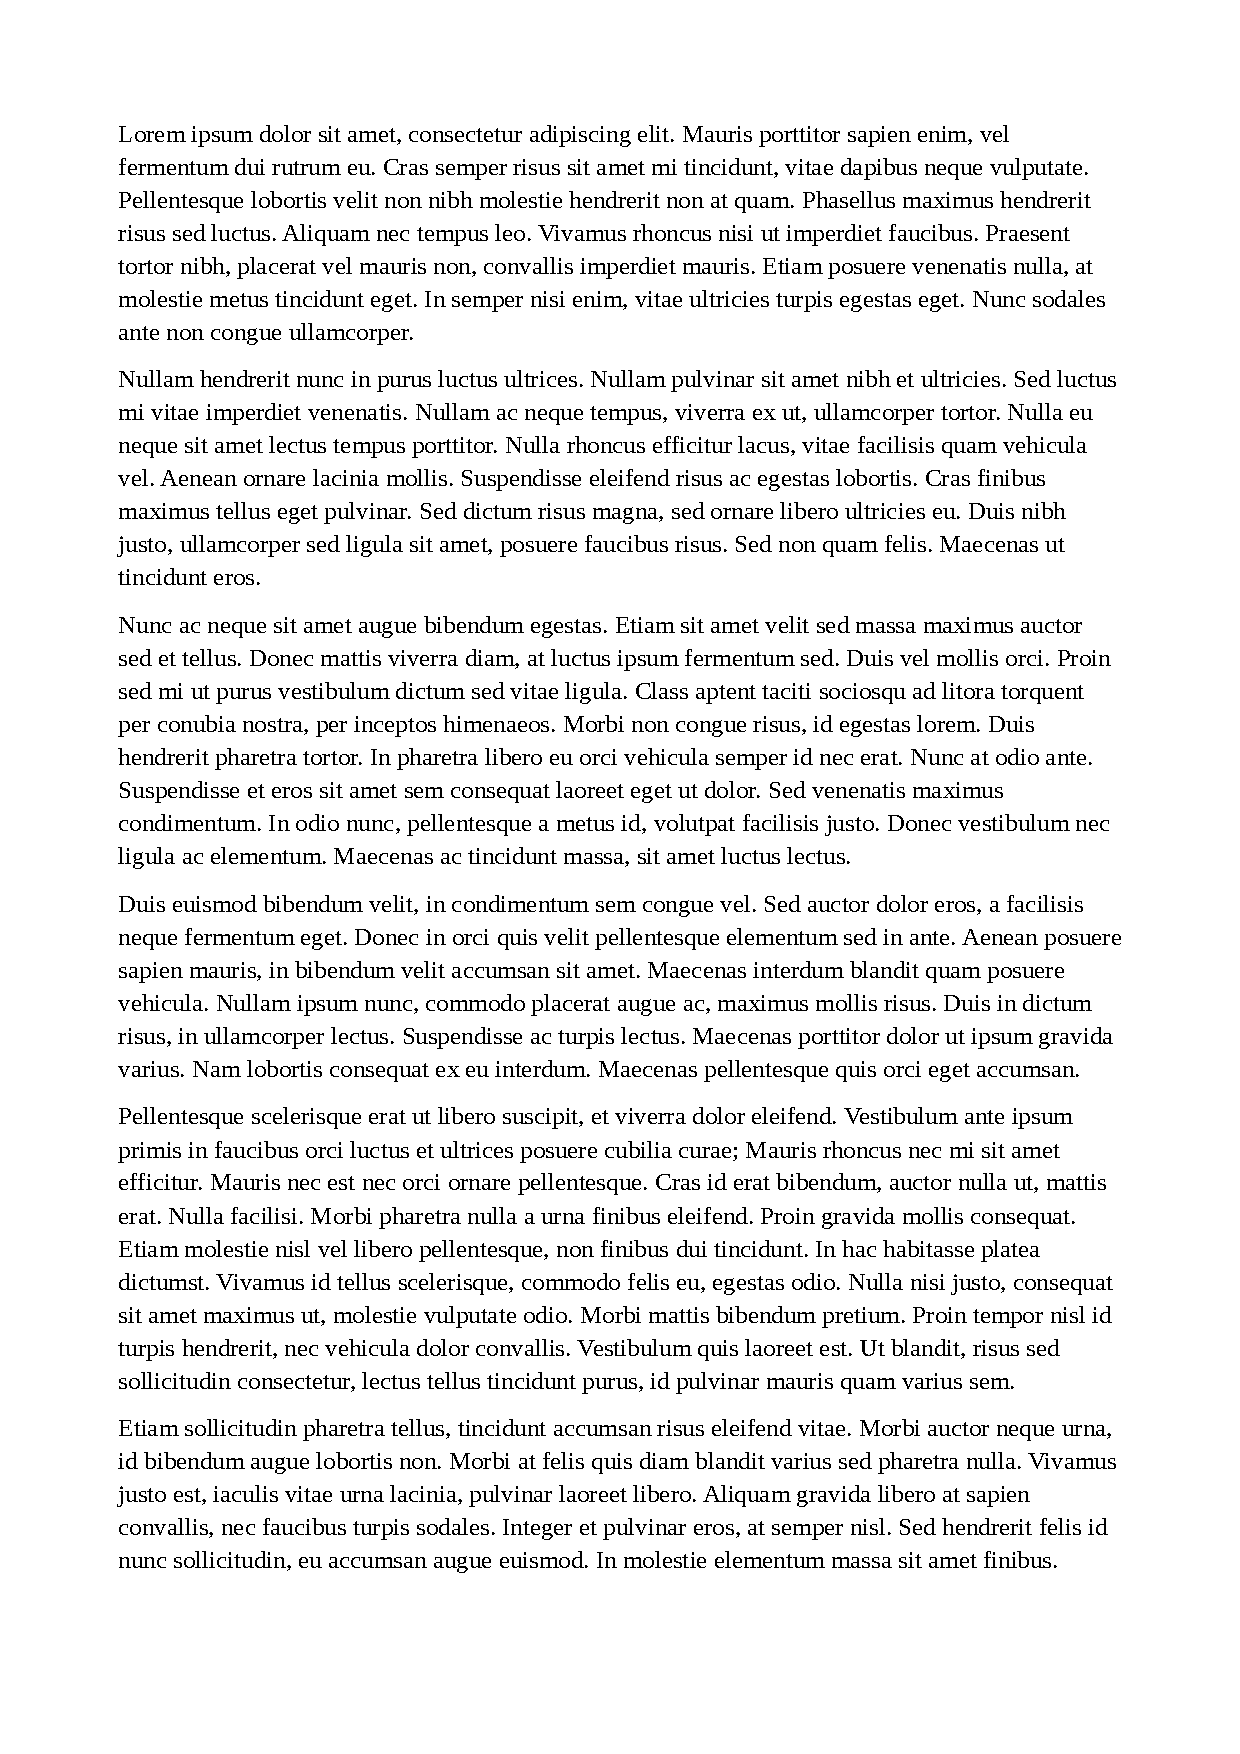
\includepdf[pages={1},scale=0.8,pagecommand=\chapter{Texto Texto Texto Texto}\label{apen:apendiceA}]{appendix/apendiceA}
\includepdf[pages={2-},scale=0.80,pagecommand={}]{appendix/apendiceA}

%coloca o identificador do anexo/apendice somente na primeira página

\includepdf[pages={1},scale=0.80,pagecommand=\chapter{Texto Texto Texto}\label{apen:apendiceB}]{appendix/apendiceB}


%coloca o identificador do anexo/apendice somente na primeira página
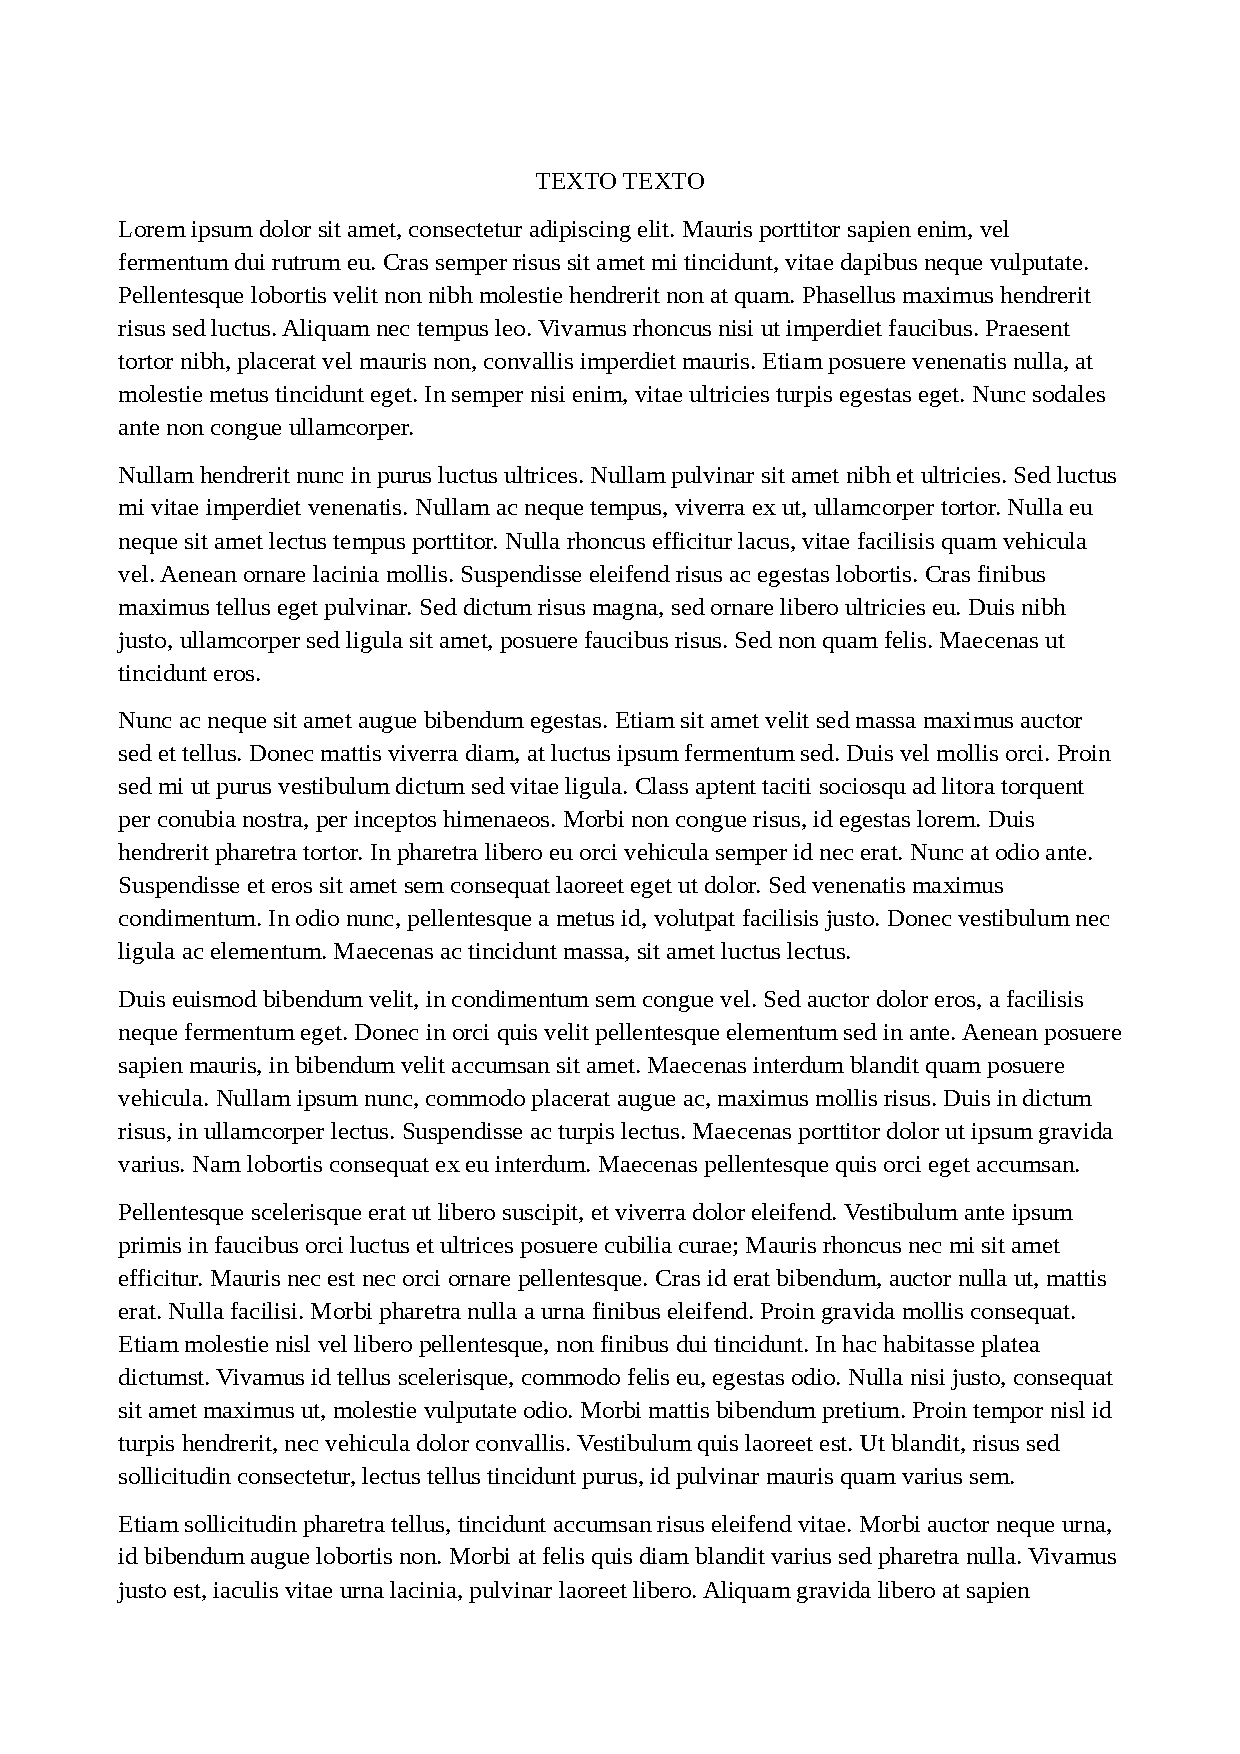
\includepdf[pages={1},scale=0.80,pagecommand=\chapter{Texto Texto}\label{apen:apendiceC}]{appendix/apendiceC}
\includepdf[pages={2},scale=0.80,pagecommand={}]{appendix/apendiceC}


\addtocontents{toc}{\endgroup}
\end{apendicesenv}




% ----------------------------------------------------------
% Anexos
% ----------------------------------------------------------
% Anexos

%%coloca o identificador do anexo/apendice somente na primeira página
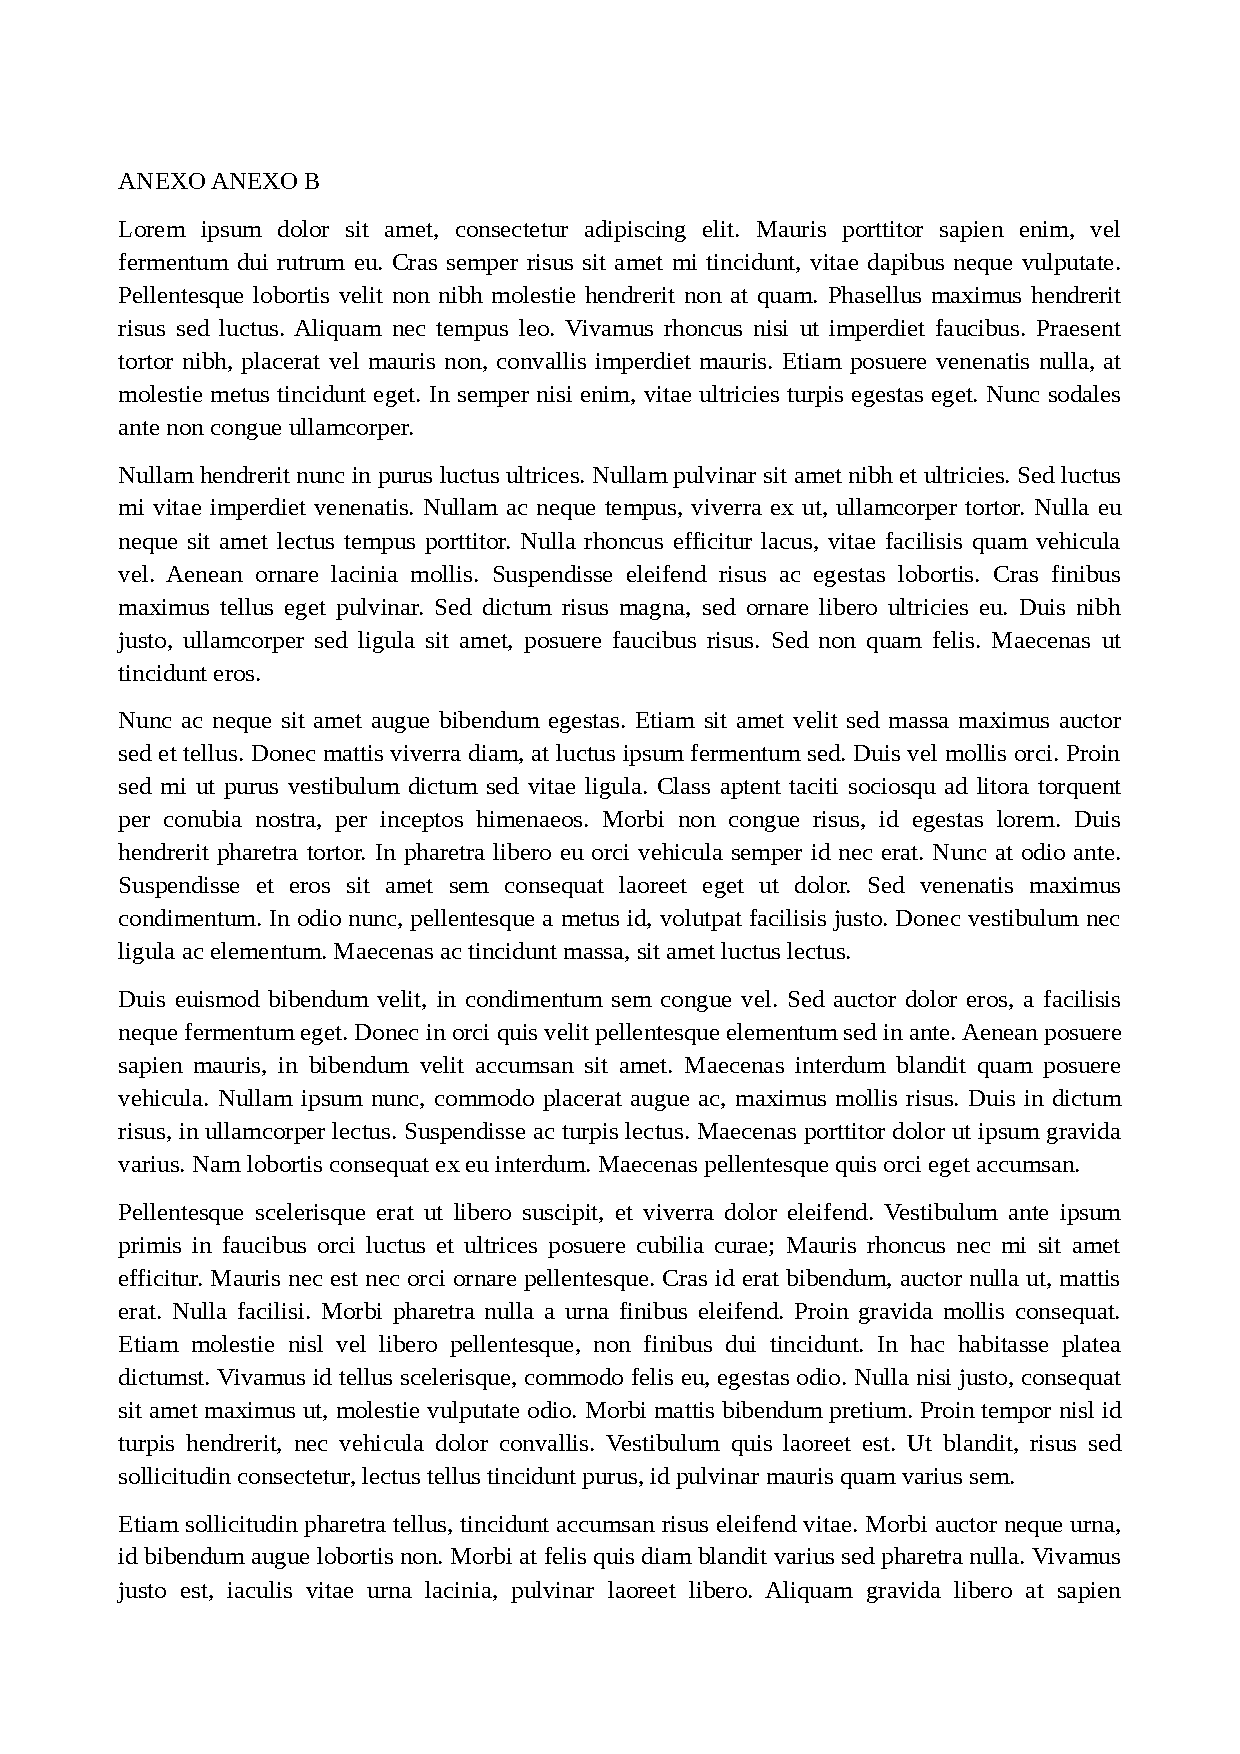
\includepdf[pages={1},scale=0.8,pagecommand=\chapter{Texto Texto Texto Texto}\label{anex:anexob}]{anexos/anexoB}
\includepdf[pages={2-},scale=0.80,pagecommand={}]{anexos/anexoB}

%%coloca o identificador do anexo/apendice somente na primeira página
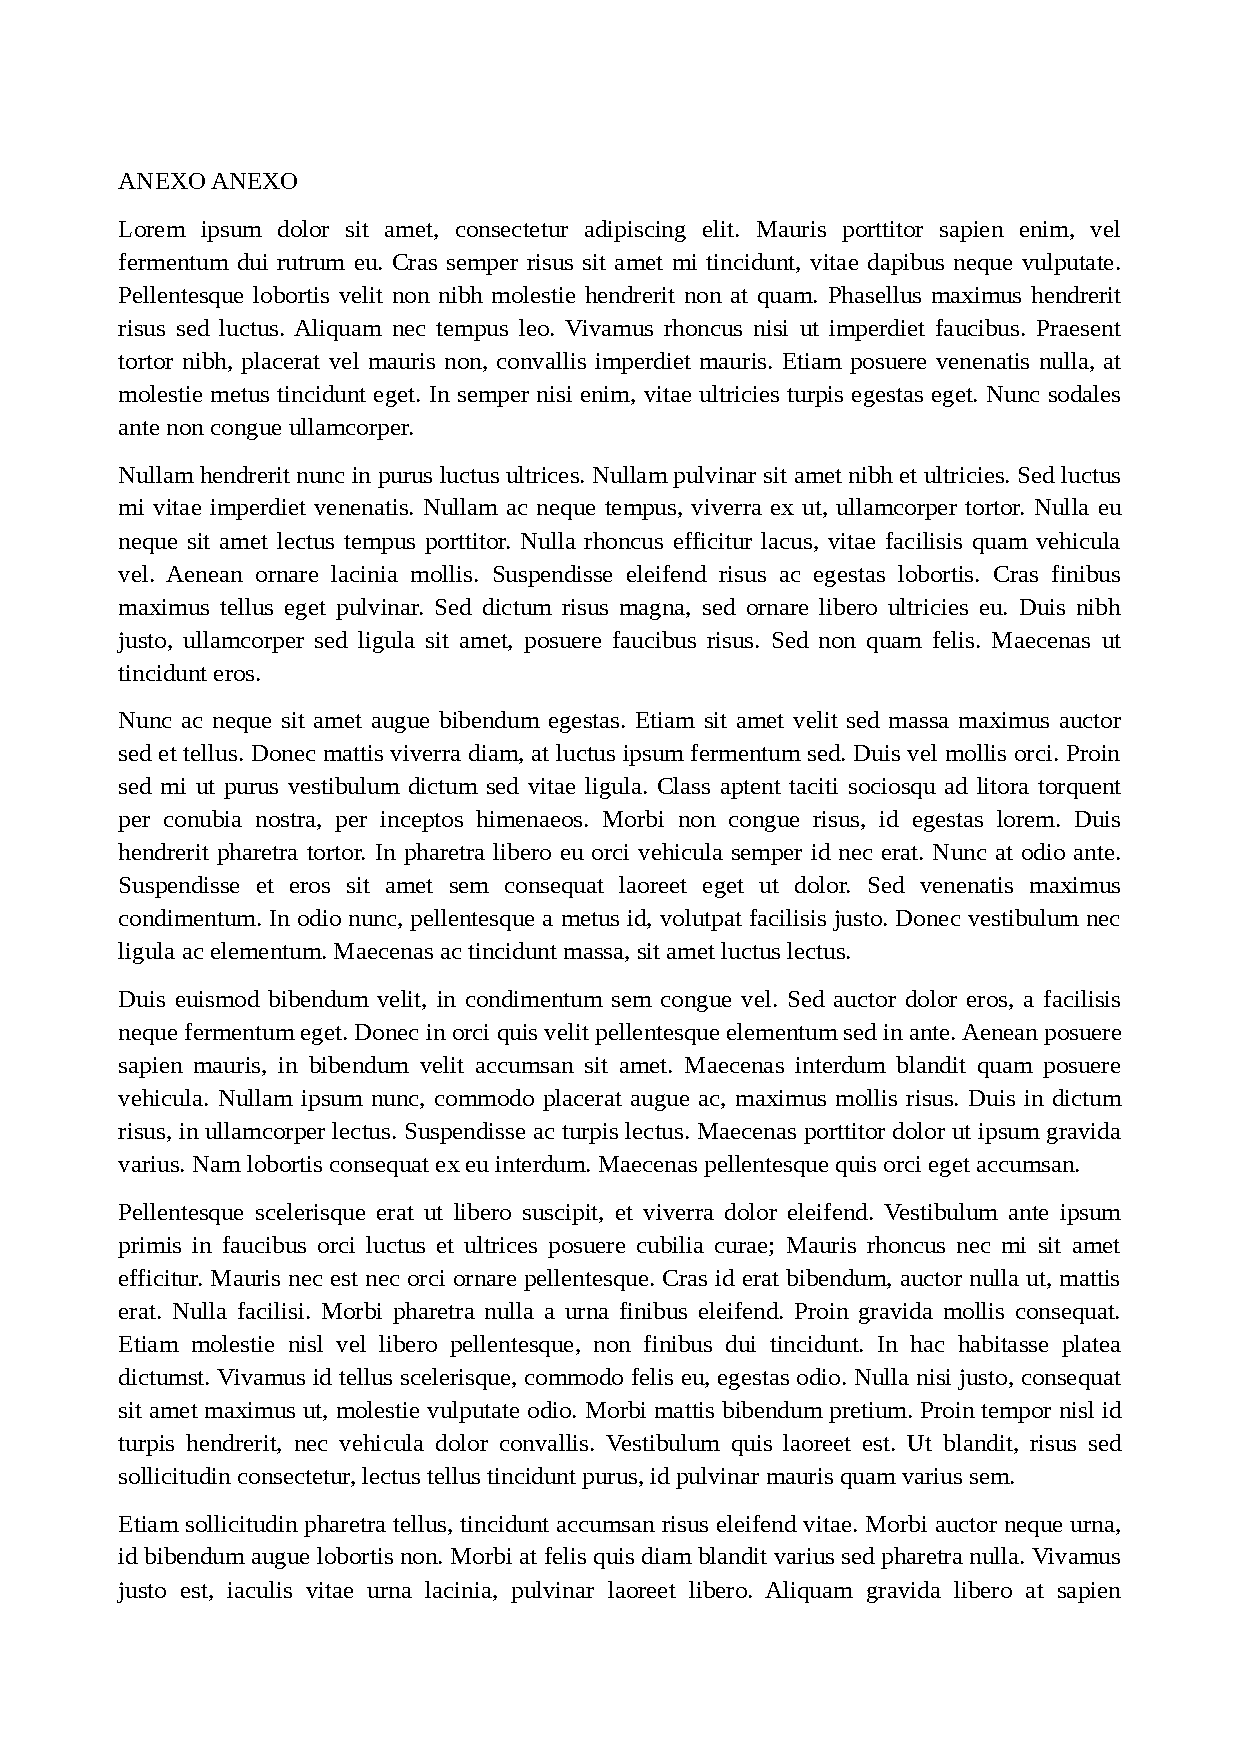
\includepdf[pages={1},scale=0.8,pagecommand=\chapter{Texto Texto Texto Texto}\label{anex:anexoa}]{anexos/anexoA}
\includepdf[pages={2-},scale=0.80,pagecommand={}]{anexos/anexoA}


\printindex


\end{document}
